\subsection{Why Objectives Help}
\label{sec:exp-why}

The objective ablation in Section~\ref{sec:exp-objectives} shows that objectives differ widely in how much they help. Here we identify the property that explains this: how class-relevant the objective's target is. For each objective with a per-node target, we fit a logistic-regression probe that predicts a node's class from the objective's target alone, and measure the probe's macro-F1 as a proxy for the class-relevance of that target. We then relate it to the objective's downstream lift from Section~\ref{sec:exp-objectives}. Relational objectives (path, triplet), whose target is a relation between sampled nodes rather than a per-node vector, are excluded from this analysis.

Figure~\ref{fig:probe-vs-lift} plots the two quantities. The more class-relevant an objective's target, the more it improves downstream classification: the neighbor label-histogram (hist) has both the most class-relevant target and the largest lift, whereas the neighbor-spread target (stats) is the least class-relevant and is the only objective that does not help. Feature reconstruction (recon) also provides a useful signal, consistent with our prior work on feature-based self-supervision for imputation~[NCSSL]. This explains why the label-aware histogram is the most reliable objective, and why we pair it with a structural objective in NESS.

The training dynamics corroborate this picture. Figure~\ref{fig:loss-curves} plots the per-objective self-supervised loss over training. Feature-space objectives with low-variance targets fall to a small value within a few epochs and then remain flat, providing little further gradient, while the label and structural objectives begin at a higher loss and continue to decrease throughout training, supplying informative supervision for longer. An objective is therefore useful when its target is both class-relevant and non-trivial to fit.

Finally, we verified that a class-irrelevant objective cannot be made useful by tuning: for a structural distance objective whose target is only weakly class-relevant, neither increasing its loss weight, adding a projection head between the encoder and the objective, nor scheduling the objective before classification changed the outcome. The determining factor is the class-relevance of the target, not the weight or attachment of the objective.

\begin{figure}[t]
\centering
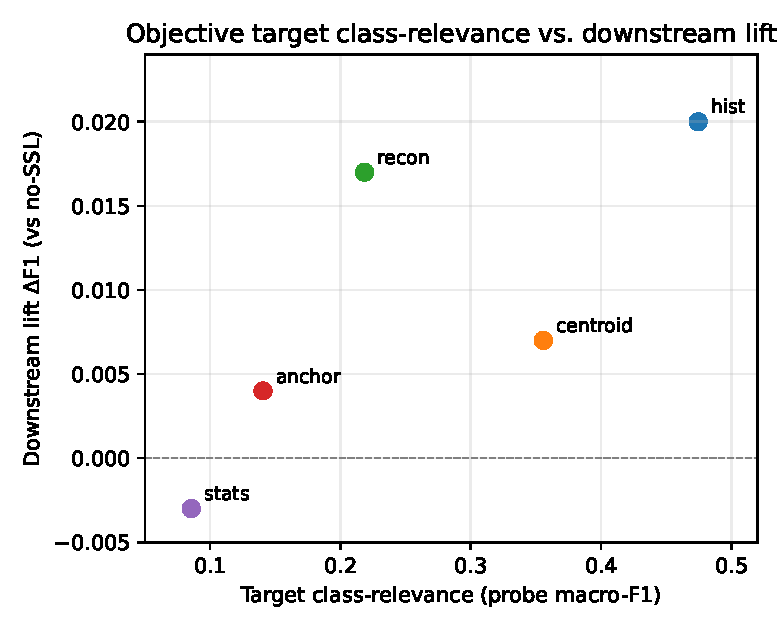
\includegraphics[width=0.85\linewidth]{figures/figA_probe_vs_lift.pdf}
\caption{Target class-relevance versus downstream lift for per-node-target objectives. Each objective's target is probed for class information (x-axis); the more class-relevant the target, the larger the downstream improvement (y-axis). The label-histogram (hist) is highest on both; the neighbor-spread target (stats) is lowest and the only one that does not help.}
\label{fig:probe-vs-lift}
\end{figure}

\begin{figure}[t]
\centering
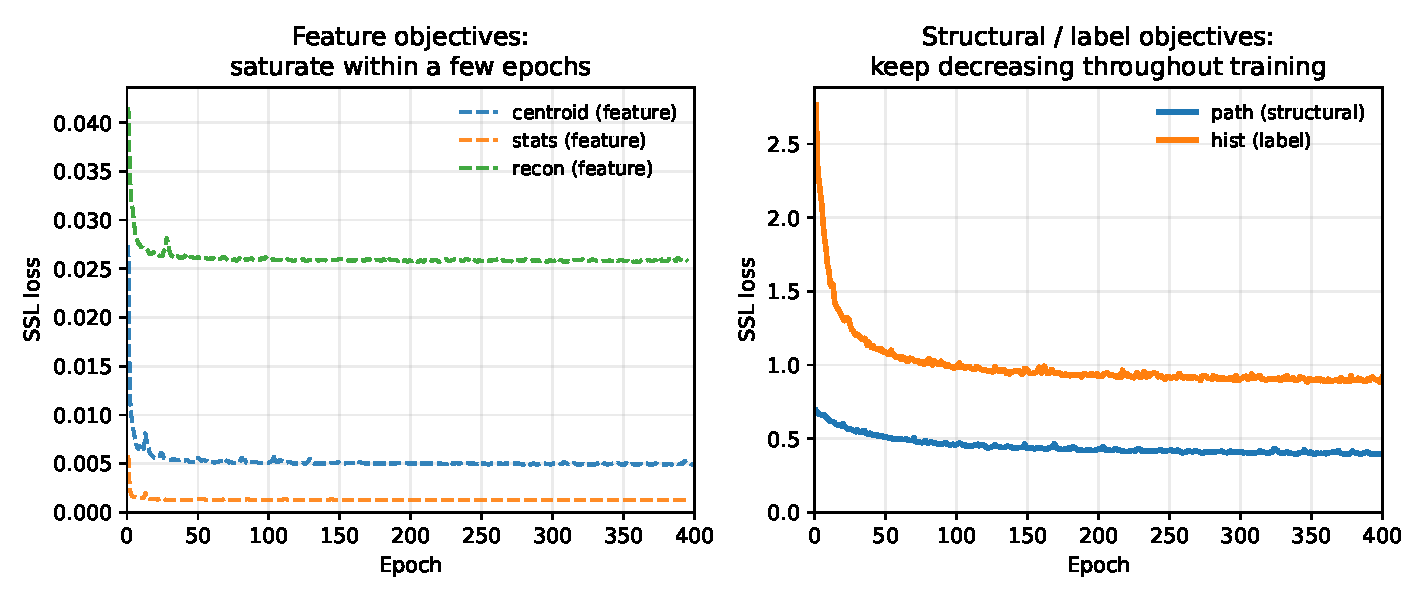
\includegraphics[width=\linewidth]{figures/e10_loss_curves.pdf}
\caption{Per-objective self-supervised loss over training (each curve from a run with that objective alone; $x$ capped at 400 epochs). Left: feature objectives saturate within a few epochs. Right: structural and label objectives keep decreasing throughout training. Axes are per-panel to make each group's shape visible.}
\label{fig:loss-curves}
\end{figure}
